        \chapter{Vassiliev Invariants and Chord Diagrams}
        \label{ch:formality-and-chord-diagrams}

        \scaffold{Filtered structures, associated graded structures, formality and how this leads to conections between Vassiliev Invariants and quantum algebra via a general application of Von Dyck's Theorem. Can include intro to PaT Vassiliev filatration, chord diagrams, Drinfeld Associators on a story sort of level.}


        \scaffold{In more detail. A section will be on chord diagrams and the associated graded. Since the introduction comes from the Vassiliev history space-of-knots point-of-view, I want to do things pretty formally with respect to the associated graded space. i.e. I don't want to say double point = overcrossing - undercrossing, as these two things are definitely not equal, but it is okay to say V(d.p.) = V(over) - V(under). To do this requires the treatment in \cite{the-fundamental-theorem-of-vassiliev-invariants}, which on the bright side means I get to talk about the polynomials analogy. It means that the statement becomes \[\text{weight systems} = \operatorname{gr}(\text{Vassiliev invariants})\] instead of directly \[\text{chord diagrams} = \operatorname{gr}(\text{singular knots})\] (or at least that's how it's put in \cite{the-fundamental-theorem-of-vassiliev-invariants}, but perhaps this can also be turned into a statement without all the implicit duals.}

        As we saw in the introduction, the knots are the connected components of the infinite-dimensional vector space of smooth maps \(S^{1} \to \R^{3}\), stratified by the codimension one subspace of 

        \scaffold{\[\uparrow \text{ new}\] \[\downarrow \text{ old}\]}

        In \cite{on-the-vassiliev-knot-invariants} Bar-Natan makes the following analogy between knot theory and calculus: two knots that differ only by a single crossing such as
        \[(1)\]
        are `close' to each other in the sense of being close in the space of smooth maps \(S^{1} \to \R^{3}\) from the introduction. This space includes the \(m\)-singular knots:
        \begin{definition}[\(n\)-singular knot]
                An \(m\)-singular knot is a singular knot (smooth map \(S^{1} \to \R^{3}\)) whose only singularities are exactly \(m\) transverse double points.
        \end{definition}

        Indeed any knot invariant \(V\) can be extended to a function \(V^{m}\) of \(m\)-singular knots \(m\) transverse double points by the formula
        \[V^{(0)} = V\]
        \[V^{(m + 1)}\left(\singular\right) = V^{(m)}\left(\poscross\right) - V^{(m)}\left(\negcross\right)\]
        The analogy stems from treating this evaluation of an invariant on two very close knots as derivative.

        Just as polynomials are the functions that vanish after a certain number of derivatives, we define:

        \begin{definition}[Vassiliev Invariant] \label{def:vassiliev_invariant}
                \begin{enumerate}[(a)]
                        \item A knot invariant is a \textit{Vassiliev invariant} of order (or type) \(m\) if
                        \[V^{(m + 1)}\biggl( \underbrace{\singular \cdots \singular}_{{\scriptscriptstyle m + 1}} \biggr) = 0.\]

                        The \textit{order} of a Vassiliev invariant \(V\) is the highest \(m\) such that \(V\) is a Vassiliev invariant of order \(m\). Equivalently, it's the highest number of double points a knot \(K\) can have without \(V(K)\) having to vanish.

                        \item The set of Vassiliev invariants of order \(m\) is a vector space, and we denote it \(\mathcal{V}_{m}\).
        \end{enumerate}
        \end{definition}

        If this analogy is worth its salt, then there should be some artefact of the calculus fact that \(f^{(m + 1)} \equiv 0\) implies \(f^{(m)}\) is a constant. This is not exactly true for Vassiliev invariants, but it is essentially true in the following sense. If
        \(V^{(m + 1)} \equiv 0\)
        then \(V^{(m)}\)
        is a collection of constants, one for each `kind' of \(m\)-singular knot that the variable
        \[\underbrace{\singular \cdots \singular}_{{\scriptscriptstyle m}}\]
        could represent. Exactly what describes a `kind' of \(m\)-singular knot will turn out to be a chord diagram, but note: other than this kind, the \(m\)th derivative of an \(m\)-singular knot does not depend on the \(m\)-singular knot, and in that sense it is a constant.

        Many well known invariants have been shown to either be Vassiliev invariants themselves, or be approximatable to arbitrary degree by a series of Vassiliev invariants. The following conjecture is the analogue of the Stone-Weierstrass theorem:
        \begin{conjecture}
                Every knot invariant can be approximated arbitrarily well by a series of Vassiliev invariants.
        \end{conjecture}
        \draftnote{Is this equivalent to Vassiliev invariants separate knots?}

        \section{Vassiliev Invariants as `Polynomials'}

        In the preamble of this chapter, we have sketched out the analogy which links Vassiliev invariants to polynomial functions. We begin to make this more precise, in the style of \cite{integration-of-singular-braid-invariants}, though the analogy will grow once we encounter formality maps (homomorphic expansions) later.



        \begin{definition}
                Let \[\mathcal{K}^{0}_{m} = \quotient{\operatorname{span}(\{m\text{-singular knots}\})}{\eqref{eq:diff_relation}}\]
                where \eqref{eq:diff_relation} is the following relation:

                \begin{equation} \label{eq:diff_relation} \tag{diff}
                        \singular \ \poscross - \singular \ \negcross = \poscross \ \singular - \negcross \ \singular
                \end{equation}
        \end{definition}

        With this definition, it doesn't matter whether an invariant is evaluated on a singular knot or its \(\delta\) image.

        The relation \eqref{eq:diff_relation} asserts that `differentiating' a knot is well-defined and independent of the crossing chosen, allowing the following definition.

        \begin{definition}
                Let \(\delta: \mathcal{K}^{0}_{m + 1} \to \mathcal{K}^{0}_{m}\) be the maps defined by
                \[\singular \longmapsto \poscross \ - \ \negcross.\]
        \end{definition}


        An important property of any \(m\)-singular knot is the cyclic order in which the double points are visited.

        \begin{definition} \label{def:chord_diagram}
                \begin{enumerate}[(a)]
                        \item A \textbf{chord diagram} of order \(m\) is an oriented circle with a distinguished set of \(m\) pairs of points, considered up to orientation-preserving diffeomorphism of the circle.
                        \item The \textbf{chord diagram of an \(n\)-singular knot}, denoted \(\sigma(K)\), is the chord diagram of order \(n\) obtained by taking the circle to be the circle in the definition of an \(n\)-singular knot as an immersion of \(S^{1}\), and the \(m\) pairs of points to be the preimages of the double points.
                        \item The \textbf{space of chord diagrams}, denoted \(\mathbf{A}_{m}\) is the linear span of all chord diagrams of order \(m\).
                \end{enumerate}
        \end{definition}

        \begin{example}
                \[\sigma \biggl( \includegraphics[width=0.14\textwidth, valign=c]{graphics/knot_9_33_singular.pdf} \biggr) =
                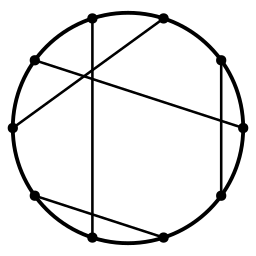
\includegraphics[width=0.13\textwidth, valign=c]{graphics/chord_diagram_of_knot_9_33_singular.pdf}\]
        \end{example}

        Let's make an important geometric observation about the space of \(m\)-singular knots.

        \begin{lemma} \label{lem:chord_diagram_crossing_change}
                The following are equivalent
                \begin{enumerate}[(a)]
                        \item Two \(m\)-singular knots \(K_{1}\) and \(K_{2}\) have the same chord diagram.
                        \item There is a sequence of \(m\)-singular knots \(K_{1}, K', K'', \cdots, K_{2}\) where consecutive knots differ by a crossing change.
                \end{enumerate}
        \end{lemma}

        \begin{proof}
                % TODO: Prove me.
        \end{proof}

        Chord diagrams as defined in definition \ref{def:chord_diagram} are geometric objects, but by the proposition below, the definition could just as well be \(m\)-singular knots modulo the images of \((m + 1)\)-singular knots.

        \begin{proposition} \label{prop:chord_diagrams_isom_singular_quotient_as_vs}
                There is a vector space isomorphism
                \[\mathcal{K}^{0}_{m} / \delta\mathcal{K}^{0}_{m + 1} \cong \mathbf{A}_{m}\]
                given by sending a class \([K] \in \mathcal{K}^{0}_{m} / \delta\mathcal{K}^{0}_{m + 1}\) to its chord diagram \(\sigma(K)\).
        \end{proposition}

        \begin{remark}
                Proposition \ref{prop:chord_diagrams_isom_singular_quotient_as_vs} should really be thought of as an alternative definition of a chord diagram, than a proposition, so we may even write \(\mathcal{K}^{0}_{m} / \delta\mathcal{K}^{0}_{m + 1} = \mathbf{A}_{m}\).
        \end{remark}

        \begin{proof}
                By lemma \ref{lem:chord_diagram_crossing_change}, if \(m\)-singular knots have the same chord diagram, they must be related by crossing changes. However, the difference between two \(m\) singular knots that are related by a crossing change is in \(\delta\mathcal{K}^{0}_{m + 1}\):
                \[\underbrace{\singular \cdots \singular}_{{\scriptscriptstyle m}} \ \poscross \ - \ \underbrace{\singular \cdots \singular}_{{\scriptscriptstyle m}} \ \negcross \ = \delta \biggl( \underbrace{\singular \cdots \singular \ \singular}_{{\scriptscriptstyle m + 1}} \biggr),\]
                so the map is injective. It is surjective as a knot with a given chord diagram can easily be constructed by adding crossings as necessary.
        \end{proof}

        % TODO: Change all (m + 1)th to m + 1st?
        This space \(\mathcal{K}^{0}_{n} / \delta\mathcal{K}^{0}_{n + 1} = \mathbf{A}_{m}\) is very important for describing Vassiliev invariants. With polynomials, when the \((m + 1)\)th derivative vanishes, the \(m\)th derivative should be a constant. With Vassiliev invariants, instead we get a series of constants, one for each chord diagram of order \(m\).

        \begin{proposition}
                To every Vassiliev invariant \(v\) of order \(m\), we can assign a linear functional on \(\mathcal{K}^{0}_{m}\) that vanishes on \(\delta \mathcal{K}^{0}_{m + 1}\), that is an element of \((\mathbf{A}_{m})^{\ast}\).
        \end{proposition}
        \begin{proof}
                We make use of that fact that \(\mathbf{A}_{m} = \mathcal{K}^{0}_{m} / \delta\mathcal{K}^{0}_{m + 1}\). Certainly a type \(m\) invariant \(v\) defines a functional on \(\mathcal{K}^{0}_{m}\). Since by definition a type \(m\) invariant vanishes on \(\mathcal{K}^{0}_{m + 1}\), so \(v\) vanishes on \(\delta\mathcal{K}^{0}_{m + 1}\), as \(\delta\) does not affect the value of any functional (it is only required embed \(\mathcal{K}^{0}_{m + 1}\) into \(\mathcal{K}^{0}_{m}\) so that the quotient can be taken).
        \end{proof}

        In fact, the map in the proposition above is independent of the value of \(v\) on any \((m - 1)\)-singular knot, and thus, there is a well-defined map
        \begin{align*}
                \mathcal{V}_{m} / \mathcal{V}_{m - 1} &\longrightarrow (\mathbf{A}_{m})^{\ast} \\
                [v]             & \longmapsto W.
        \end{align*}
        Just as with polynomials, when we take the \(m\)th derivative of a polynomial of degree \(m\), we recieve a (collection of) constant(s), well-defined up to the addition of any degree \(m - 1\) polynomial.

        \begin{proposition}
                Suppose that \(v\) has `\(m\)th derivative' \(W\). The collection of constants \(W \in (\mathbf{A}_{m})^{\ast}\) completely determines the value of the Vassiliev invariant \(v\) on an \(m\)-singular knot.
        \end{proposition}

        \begin{proof}
                By lemma \ref{lem:chord_diagram_crossing_change}, (and just as in the proof of proposition \ref{prop:chord_diagrams_isom_singular_quotient_as_vs}), any two \(n\)-singular knots are related by a sequence of \(n\)-singular knots, such that consecutive differences are elements of \(\delta(\mathcal{K}^{0}_{m + 1})\). But since \(v\) is of type \(m\), this is zero.
        \end{proof}


        \section{Weight Systems}

        One might hope that any collection of constants \(W \in (\mathbf{A}_{m})^{\ast}\) is obtained as the collection of differentiation constants for some order \(m\) Vassiliev invariant \(v\). Certainly this is true for polynomials, one only needs to integrate the constant \(m\) times to find a suitable polynomial. However, this is not the case for Vassiliev invariants. It is necessary for \(W\) to satisfy some equations to be `integrated'.

        \subsection{One-term relations}

        Knots are

        \scaffold{Which ones do integrate? Clearly not those that have isolated chords (1T). These ones can't become knot invariants, as \(v_{m}(\delta(K_{\text{1T}})) = v_{m}(K - K) = 0\). As we see in this way, elements of \(\ker \delta\) become relations that weight systems must satisfy to integrate. These relations on knots ("topological relations") pass down to relations on chord diagrams.}

        \scaffold{We have not discovered the whole of \(\ker \delta\).}

        \subsection{Four-term relations}

        \scaffold{The following topological relation passes down to a relation on chord diagrams. (insert 4-term relation)}

        \scaffold{Insert the stanford/hutchings/Bar-Natan thing about the exact sequence \(\mathcal{K}^{1}_{m} \xrightarrow{\partial} \mathcal{K}^{0}_{m} \xrightarrow{\delta} \mathcal{K}^{0}_{m + 1}\) and how this proves that the kernel is generated by (1T) and (4T).}

